In order to relate the calculated attenuation coefficient of a particular object to the effective energy, a $2^\text{nd}$ degree, 4 knot B-spline was used to fit NIST's mass attenuation coefficient data, where the mass attenuation coefficient is defined as the attenuation coefficient divided by the object's density, $\mu/\rho$. This fit, implemented with the Python package Scikit-Learn \cite{scikit-learn}, provided $\mu = f(E_{\text{eff}})$; however, $E_{\text{eff}} = f(\mu)$ was needed. The descibed fits are shown in figure \ref{figure:NISTSplineFit}.


\begin{figure}[htbp]
    \centering
    \subfigure[Al]{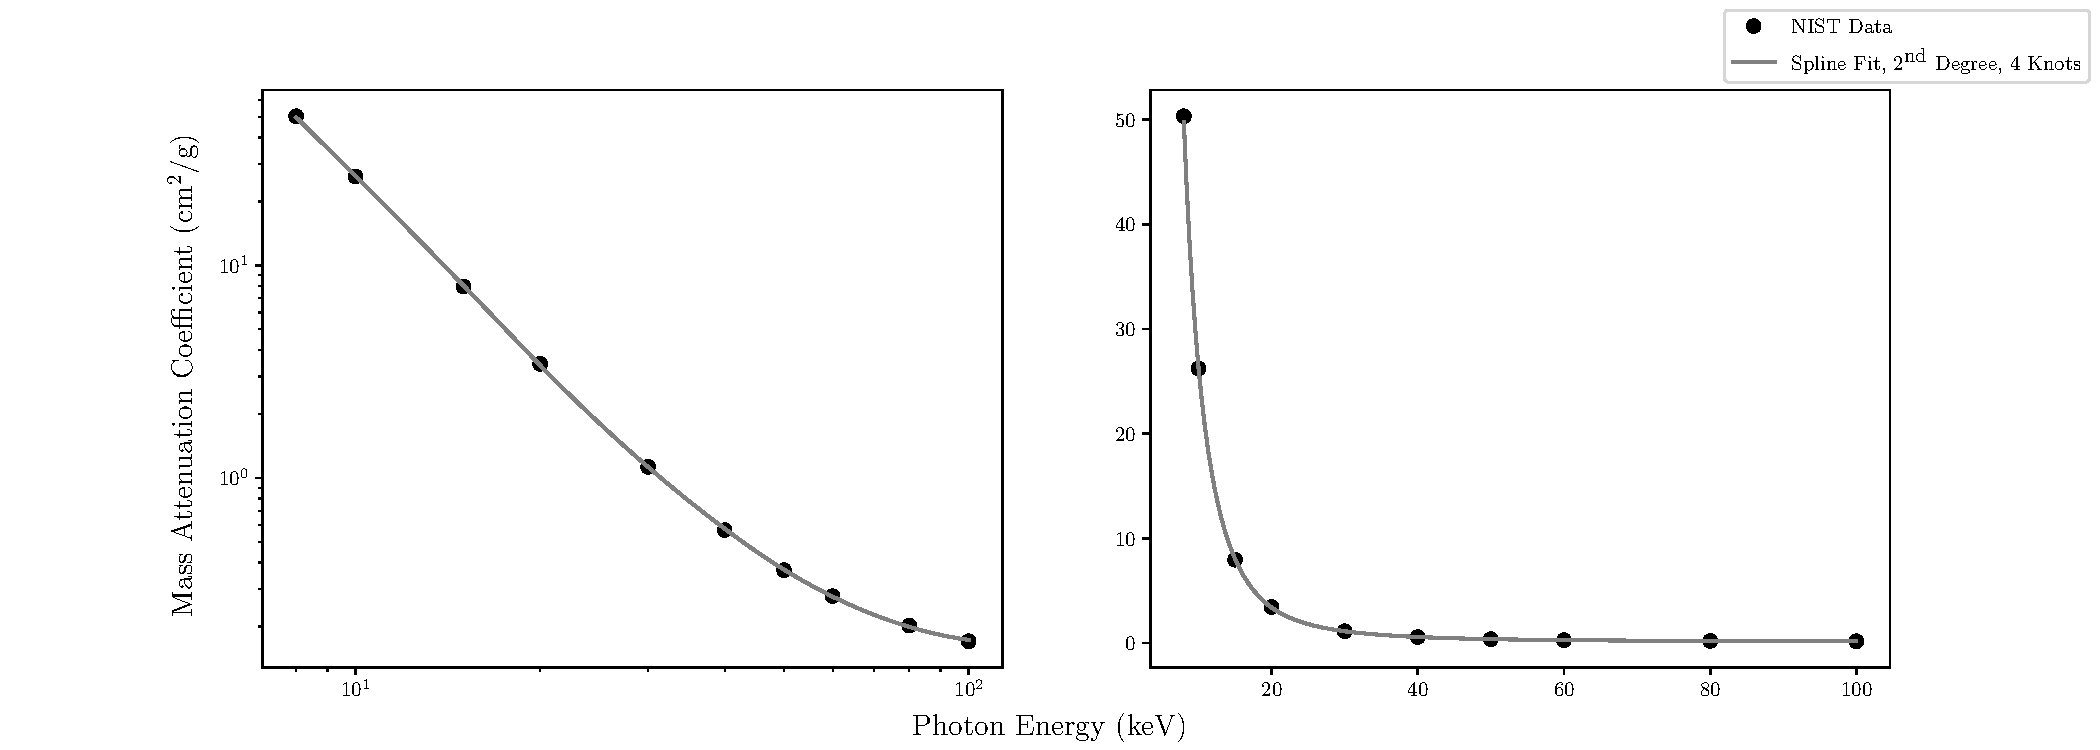
\includegraphics[width=1\linewidth]{Al_NISTSplineFit.pdf}}
    \subfigure[Fe]{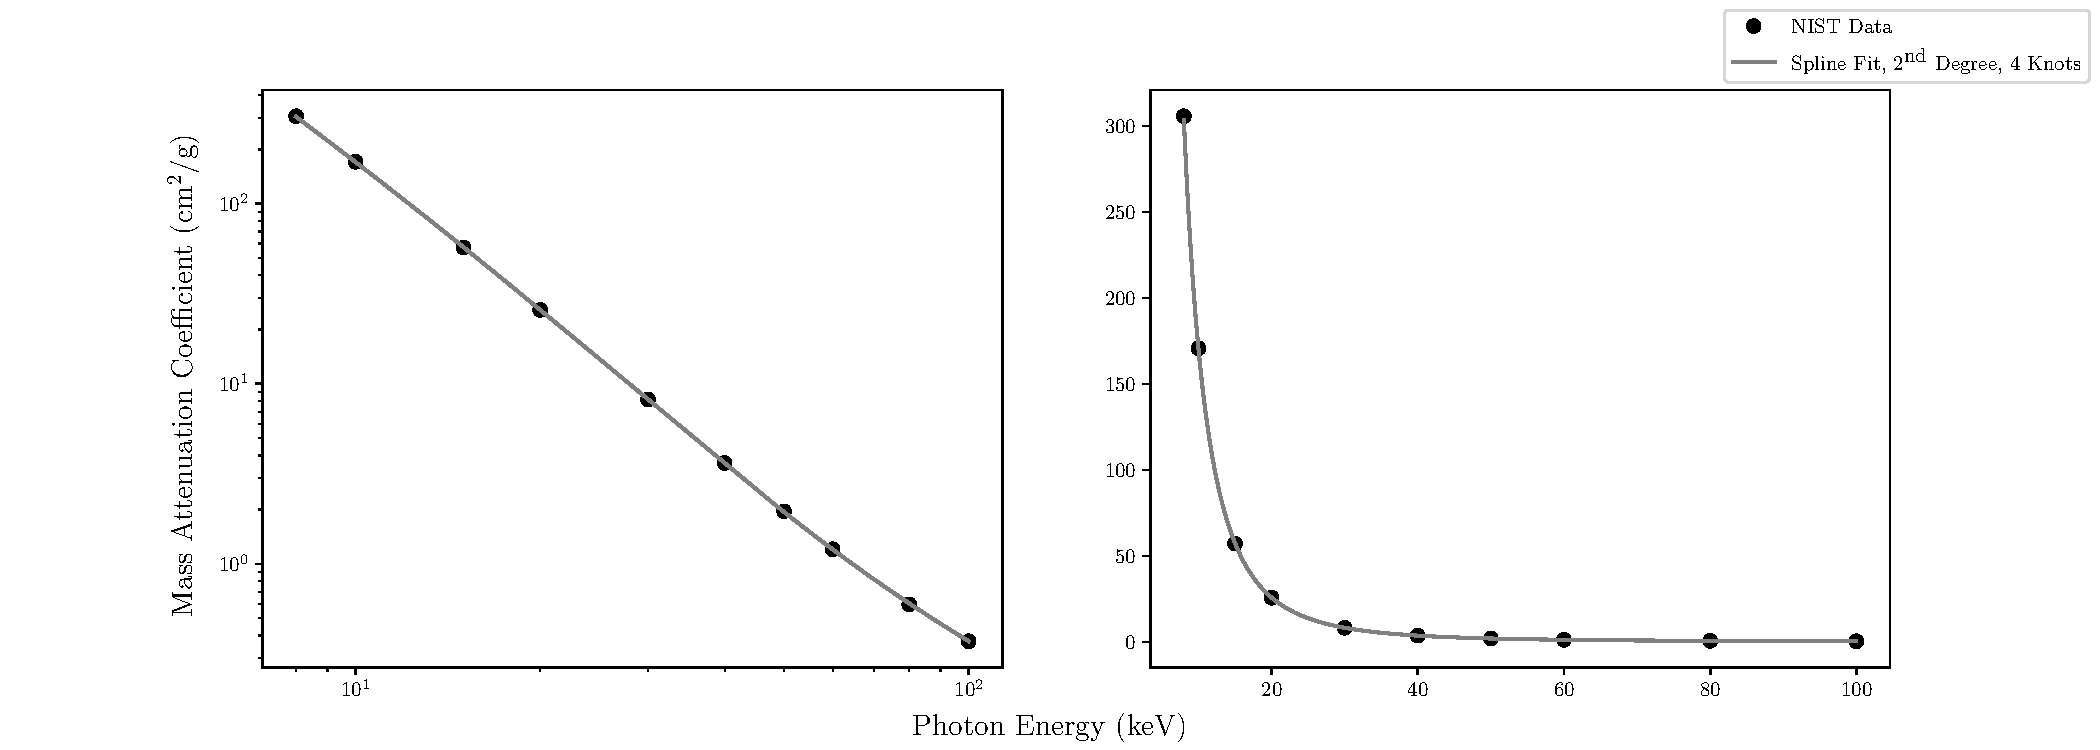
\includegraphics[width=1\linewidth]{Fe_NISTSplineFit.pdf}}
\end{figure}

\begin{figure}[htbp]
    \addtocounter{subfigure}{2}
    \ContinuedFloat
    \addtocounter{figure}{1}
    \centering
    \subfigure[Mg]{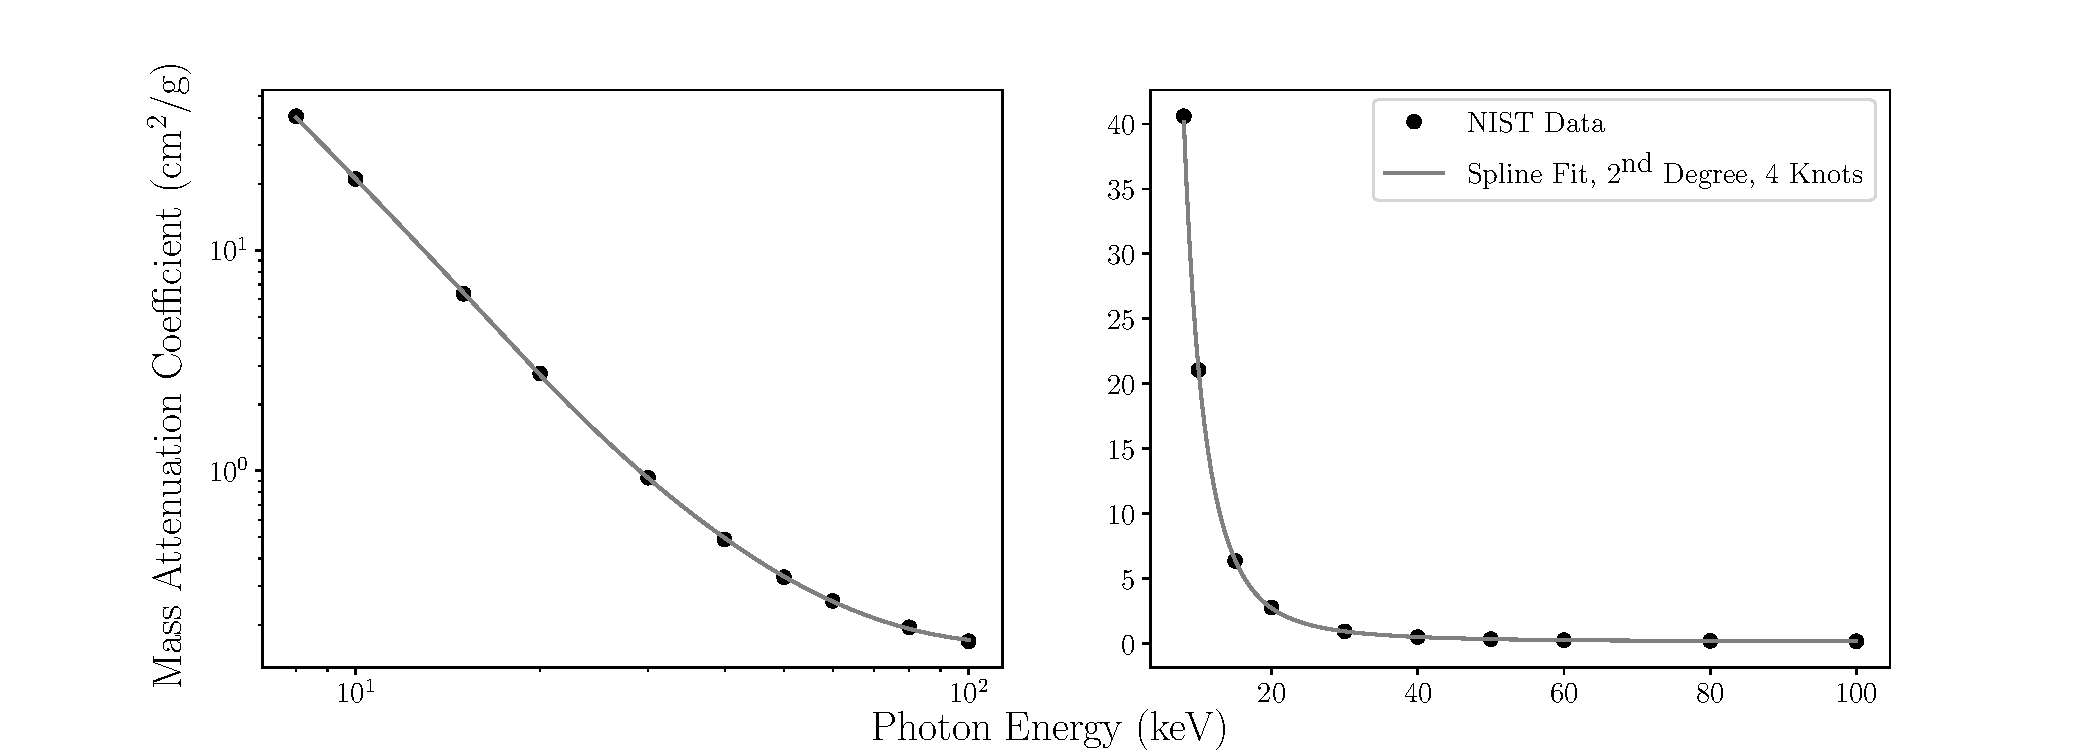
\includegraphics[width=1\linewidth]{Mg_NISTSplineFit.pdf}}
    \subfigure[Plastic Scintillator]{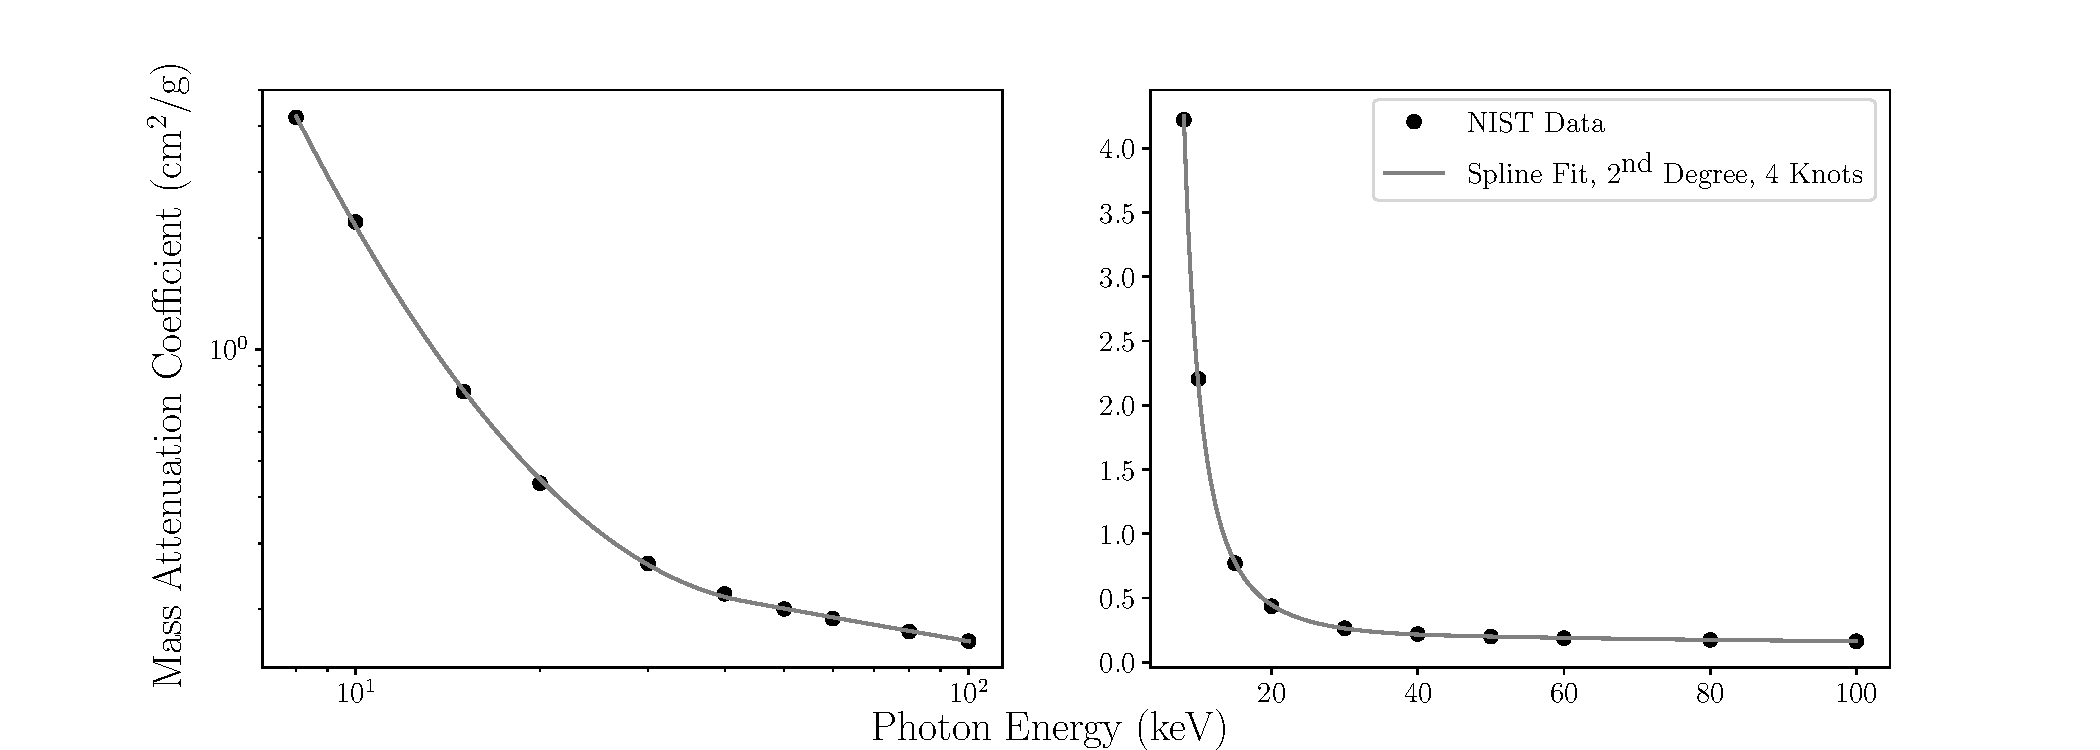
\includegraphics[width=1\linewidth]{Plastic Scintillator (Vinyltoluene-based)_NISTSplineFit.pdf}}
    \subfigure[Water]{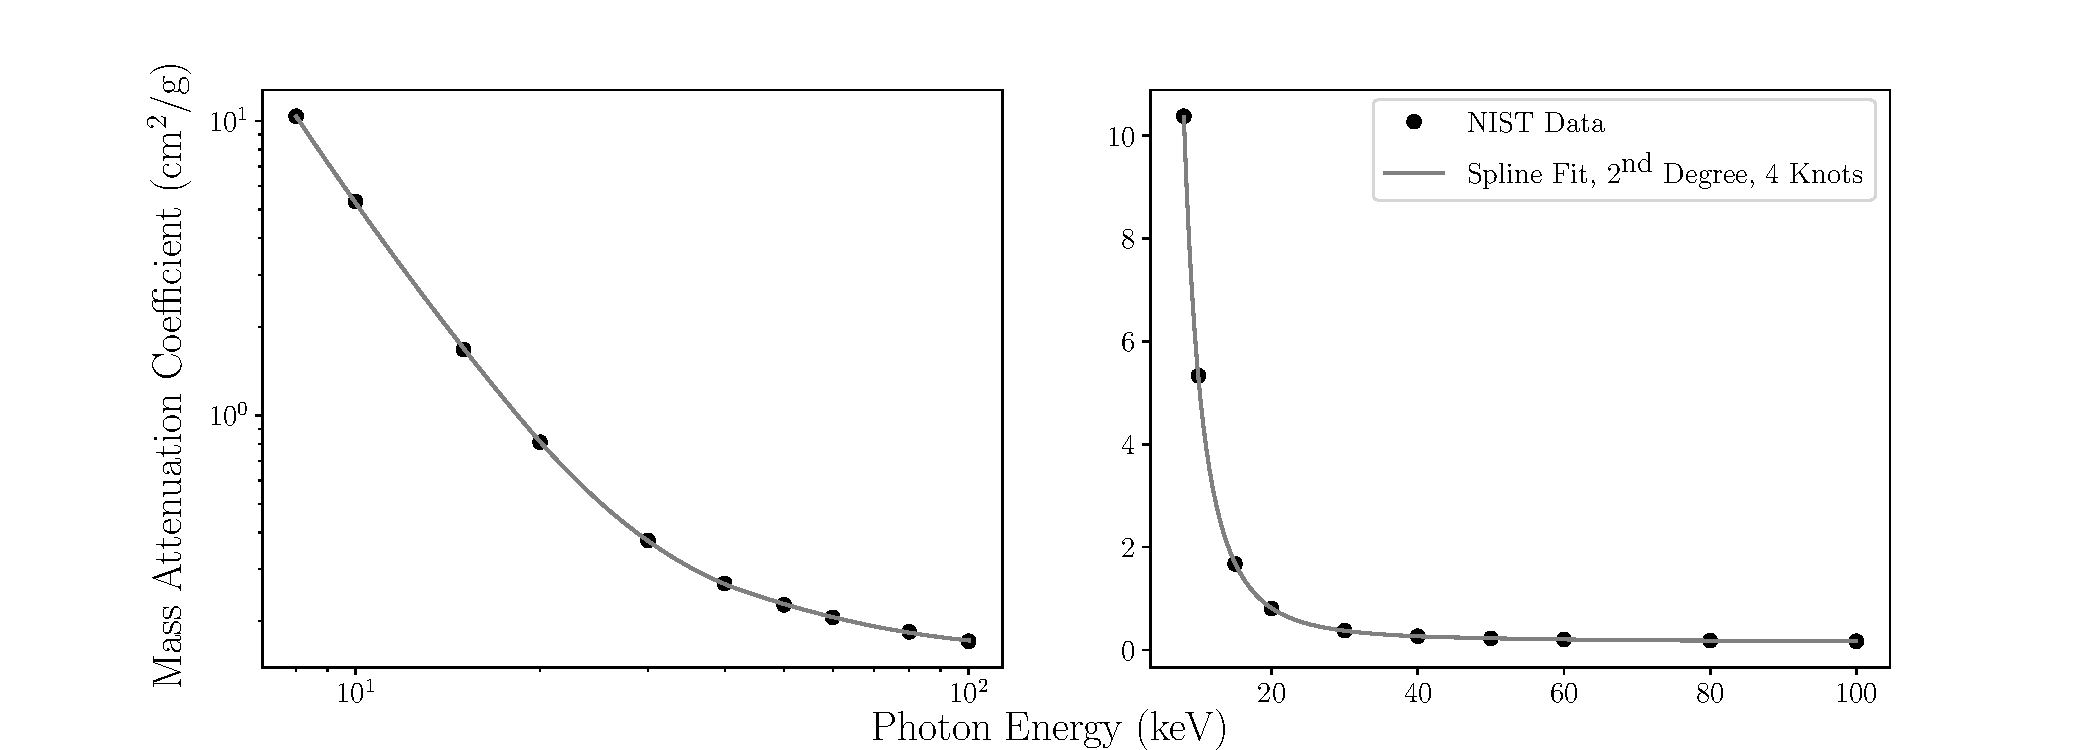
\includegraphics[width=1\linewidth]{Water, Liquid_NISTSplineFit.pdf}}
    \caption{The NIST mass attenuation coefficient (in cm$^2$/g) vs. effective energy (in keV) for the Al, Fe, Mg, Plastic Scintillator, and Water fitted using the described B-Spline.}
    \label{figure:NISTSplineFit}
\end{figure}

\newpage
Because $f$ represents an abstract model, an inverse was unable to be taken, so an evenly spaced $E_{\text{eff}}$ array of 10,000 values ranging from 0.8 keV to 100 keV was substituted into our model, providing their associated $\mu/\rho$ array. Given a particular $\mu/\rho \pm \sigma$, where $\sigma$ represents the sample standard deviation of the mass attenuation coefficient, the $E_{\text{eff}}$ was found by first determining the index of the element in the $\mu/\rho$ array closest to the particular $\mu/\rho$. The associated $E_{\text{eff}}$ was then simply the element in the $E_{\text{eff}}$ array located at the determined index. The range of error for a particular $E_{\text{eff}}$ was calculated by repeating the indexing process for $\mu/\rho + \sigma$ and $\mu/\rho - \sigma$. The results of this indexing technique for each X-ray image can be found in table 1

% \begin{table}[H]
%     \centering
%     \caption{Al}
%     \resizebox{\textwidth}{!}{
%     \begin{tabular}{cccccc}
\toprule
 kVp (keV) &  $I/I_0$ &  $\sigma$ &  $E_{\text{eff}}$ (keV) &  $E_{\text{eff}}$ Max (keV) &  $E_{\text{eff}}$ Min (keV) \\
\midrule
      40.0 &               0.310 &                                  0.025 &                  24.552 &                      25.215 &                      23.954 \\
      42.0 &               0.425 &                                  0.026 &                  27.635 &                      28.444 &                      26.917 \\
      44.0 &               0.567 &                                  0.025 &                  32.576 &                      33.698 &                      31.591 \\
      46.0 &               0.668 &                                  0.023 &                  37.747 &                      39.302 &                      36.403 \\
      48.0 &               0.727 &                                  0.023 &                  42.145 &                      44.380 &                      40.277 \\
      50.0 &               0.888 &                                  0.020 &                  83.926 &                     100.000 &                      69.711 \\
\bottomrule
\end{tabular}

%     }
% \end{table}

% \begin{table}[H]
%     \centering
%     \caption{Fe}
%     \resizebox{\textwidth}{!}{
%     \begin{tabular}{cccccc}
\toprule
 kVp (keV) &  $I/I_0$ &  $\sigma$ &  $E_{\text{eff}}$ (keV) &  $E_{\text{eff}}$ Max (keV) &  $E_{\text{eff}}$ Min (keV) \\
\midrule
      40.0 &               0.353 &                                  0.030 &                  25.316 &                      26.089 &                      24.626 \\
      42.0 &               0.432 &                                  0.031 &                  27.331 &                      28.196 &                      26.558 \\
      44.0 &               0.595 &                                  0.030 &                  32.392 &                      33.588 &                      31.352 \\
      46.0 &               0.678 &                                  0.027 &                  35.870 &                      37.287 &                      34.646 \\
      48.0 &               0.761 &                                  0.028 &                  40.599 &                      42.687 &                      38.860 \\
      50.0 &               0.911 &                                  0.024 &                  60.335 &                      69.195 &                      54.704 \\
\bottomrule
\end{tabular}

%     }
% \end{table}

% \begin{table}[H]
%     \centering
%     \caption{Mg}
%     \resizebox{\textwidth}{!}{
%     \begin{tabular}{cccccc}
\toprule
 kVp (keV) &  Relative Intensity &  Relative Intensity Standard Deviation &  Effective Energy (keV) &  Effective Energy Max (keV) &  Effective Energy Min (keV) \\
\midrule
      40.0 &               0.632 &                                  0.030 &                  20.200 &                      20.982 &                      19.529 \\
      42.0 &               0.832 &                                  0.029 &                  28.444 &                      31.058 &                      26.531 \\
      44.0 &               0.874 &                                  0.027 &                  32.382 &                      36.412 &                      29.668 \\
      46.0 &               0.909 &                                  0.027 &                  37.967 &                      46.193 &                      33.431 \\
      48.0 &               0.940 &                                  0.024 &                  48.162 &                      72.627 &                      39.936 \\
\bottomrule
\end{tabular}

%     }
% \end{table}




% \begin{table}[H]
%     \centering
%     \caption{Plastic Scintillator}
%     \resizebox{\textwidth}{!}{
%     \begin{tabular}{cccccccc}
\toprule
 kVp (kV) &  $I/I_0$ &  $I/I_0$ Std. &  $\mu/\rho$ (cm$^2$/g) &  $\mu/\rho$ Std. (cm$^2$/g) &  $E_{\text{eff}}$ (keV) &  $E_{\text{eff}}$ Max (keV) &  $E_{\text{eff}}$ Min (keV) \\
\midrule
     40.0 &    0.578 &          0.03 &                  0.268 &                       0.025 &                  29.392 &                      32.861 &                      27.000 \\
     42.0 &    0.645 &          0.03 &                  0.215 &                       0.023 &                  40.341 &                      57.906 &                      33.845 \\
\bottomrule
\end{tabular}

%     }
% \end{table}

% \begin{table}[H]
%     \centering
%     \caption{Water}
%     \resizebox{\textwidth}{!}{
%     \begin{tabular}{cccccc}
\toprule
 kVp (keV) &  $I/I_0$ &  $\sigma$ &  $E_{\text{eff}}$ (keV) &  $E_{\text{eff}}$ Max (keV) &  $E_{\text{eff}}$ Min (keV) \\
\midrule
      44.0 &               0.059 &                                  0.025 &                  25.500 &                      28.076 &                      23.669 \\
      46.0 &               0.220 &                                  0.030 &                  41.096 &                      46.984 &                      37.369 \\
      48.0 &               0.325 &                                  0.029 &                  68.652 &                      86.603 &                      58.403 \\
\bottomrule
\end{tabular}

%     }
% \end{table}

\begin{table}[H]
    \small
    \noindent\makebox[\textwidth]{%
    \begin{tabularx}{1.27\textwidth}{CCCCCCCCC}

    \toprule
    Material & kVp (kV) &  $I/I_0$ &  $I/I_0$ Std. &  $\mu/\rho$ (cm$^2$/g) &  $\mu/\rho$ Std. (cm$^2$/g) &  $E_{\text{eff}}$ (keV) &  $E_{\text{eff}}$ Max (keV) &  $E_{\text{eff}}$ Min (keV) \\
    \midrule
    & 40.0 &    0.310 &         0.025 &                  1.895 &                       0.131 &                  24.552 &                      25.215 &                      23.954 \\
    & 42.0 &    0.425 &         0.026 &                  1.385 &                       0.099 &                  27.635 &                      28.444 &                      26.917 \\
    Aluminum& 44.0 &    0.567 &         0.025 &                  0.920 &                       0.071 &                  32.576 &                      33.698 &                      31.591 \\
    & 46.0 &    0.668 &         0.023 &                  0.655 &                       0.056 &                  37.747 &                      39.302 &                      36.403 \\
    & 48.0 &    0.727 &         0.023 &                  0.516 &                       0.052 &                  42.145 &                      44.380 &                      40.277 \\
    & 50.0 &    0.888 &         0.020 &                  0.192 &                       0.037 &                  83.926 &                     100.000 &                      69.711 \\
    \midrule
    & 40.0 &    0.353 &         0.030 &                 13.239 &                       1.078 &                  25.316 &                      26.089 &                      24.626 \\
    & 42.0 &    0.432 &         0.031 &                 10.668 &                       0.898 &                  27.331 &                      28.196 &                      26.558 \\
    Iron& 44.0 &    0.595 &         0.030 &                  6.595 &                       0.642 &                  32.392 &                      33.588 &                      31.352 \\
    & 46.0 &    0.678 &         0.027 &                  4.937 &                       0.514 &                  35.870 &                      37.287 &                      34.646 \\
    & 48.0 &    0.761 &         0.028 &                  3.473 &                       0.461 &                  40.599 &                      42.687 &                      38.860 \\
    & 50.0 &    0.911 &         0.024 &                  1.186 &                       0.340 &                  60.335 &                      69.195 &                      54.704 \\
    \midrule
    & 40.0 &    0.632 &         0.030 &                  2.638 &                       0.274 &                  20.200 &                      20.982 &                      19.529 \\
    & 42.0 &    0.832 &         0.029 &                  1.054 &                       0.200 &                  28.444 &                      31.058 &                      26.531 \\
    Magnesium& 44.0 &    0.874 &         0.027 &                  0.776 &                       0.176 &                  32.382 &                      36.412 &                      29.668 \\
    & 46.0 &    0.909 &         0.027 &                  0.551 &                       0.172 &                  37.967 &                      46.193 &                      33.431 \\
    & 48.0 &    0.940 &         0.024 &                  0.353 &                       0.145 &                  48.162 &                      72.627 &                      39.936 \\
    \midrule
    Plastic& 40.0 &    0.578 &          0.03 &                  0.268 &                       0.025 &                  29.392 &                      32.861 &                      27.000 \\
    Scintillator& 42.0 &    0.645 &          0.03 &                  0.215 &                       0.023 &                  40.341 &                      57.906 &                      33.845 \\
    \midrule
    & 44.0 &    0.059 &         0.025 &                  0.489 &                       0.075 &                  25.500 &                      28.076 &                      23.669 \\
    Water & 46.0 &    0.220 &         0.030 &                  0.261 &                       0.024 &                  41.096 &                      46.984 &                      37.369 \\
    & 48.0 &    0.325 &         0.029 &                  0.194 &                       0.015 &                  68.652 &                      86.603 &                      58.403 \\
    \bottomrule
\end{tabularx}
    }
    \caption{test}
\end{table}



The graphs of the $E_{\text{eff}}$ for each kVp and material combination is found in figure 4. In order to compare the experimental results, simulated $E_{\text{eff}}$ values were obtained with the Python module SpekPy \cite{SpekPy}, using the X-ray tube assembly specifications as provided by the manufacturer \cite{CArm}.


\begin{figure}[H]
    \centering
    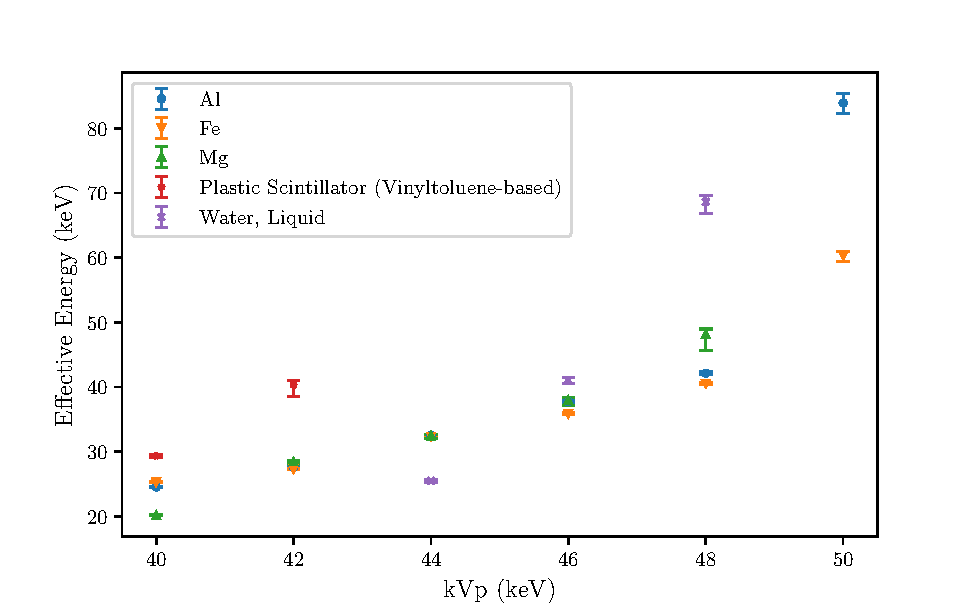
\includegraphics[width=1\linewidth]{effEnergy.pdf}
    \caption{}
\end{figure}

Figure 4 shows relative agreement and an approximately linear increase for the Al, Fe, and Mg, up until 50 kVp, where a sudden spike in $E_{\text{eff}}$ is observed. For the plastic scintillator and water, vastly different values are observed. Upon further inspection by increasing the range of the fit shown in figure 3, the two values increase at an exponential rate. Furthermore, only a few values agree with the simulation; the rate of increase of $E_{\text{eff}}$ with respect to kVp is greater for the experimental values.

For the offset experiment, the intensity values for the image with the centered Al was obtained with the standard pipeline that was used for all other images. On the other hand, the intensity values for the image with the offsetted Al were obtained manually using the software ImageJ \cite{ImageJ}.


\begin{table}[H]
    \small
    \noindent\makebox[\textwidth]{%
    \begin{tabularx}{1.15\textwidth}{cccccccc}
    \toprule
    Position & $I/I_0$ &  $I/I_0$ Std. &  $\mu/\rho$ (cm$^2$/g) &  $\mu/\rho$ Std. (cm$^2$/g) &  $E_{\text{eff}}$ (keV) &  $E_{\text{eff}}$ Max (keV) &  $E_{\text{eff}}$ Min (keV) \\
    \midrule
    Center   &  0.310   &   0.025       &   1.90                &   0.13                        &   24.55                &  25.21                       &   24.00 \\
    Offset   &  0.14    &   0.05        &   3.2                 &   0.5                         &   20.5                 &  21.9                        &   19.4  \\
    \bottomrule
\end{tabularx}               

    }
    \caption{test}
\end{table}

Table 2 shows unexpected discrepancies between the centered and offsetted Al. A slight difference is expected due to the point-like nature of the x-ray source; however, it can not explain the large difference observed due to the large distance (44.95 cm) between the x-ray source and detector.


For the thickness varying experiment, x-ray images of Al were taken at 40 kVp. The thickness of the Al was varied by using two different attenuators, one of thickness 2.286 mm and the other of thickness 0.813 mm. The intensity values for each image was obtained with the standard pipeline that was used for all other images.

\begin{table}[H]
    \small
    \noindent\makebox[\textwidth]{%
    \begin{tabularx}{1.2\textwidth}{CCCCCCCC}
    \toprule
    Thickness (mm) & $I/I_0$ &  $I/I_0$ Std. &  $\mu/\rho$ (cm$^2$/g) &  $\mu/\rho$ Std. (cm$^2$/g) &  $E_{\text{eff}}$ (keV) &  $E_{\text{eff}}$ Max (keV) &  $E_{\text{eff}}$ Min (keV) \\
    \midrule
    2.286          & 0.310   &  0.025        &  1.90                  &     0.13                    &   24.55                 &     25.21                   &   24.00   \\
    0.813          & 0.575   &  0.029        &  2.52                  &     0.23                    &   22.15                 &     22.92                   &   21.39   \\
    \bottomrule
\end{tabularx}
    }
    \caption{test}
\end{table}

While we expect 














